\chapter{Validation and improvement of the MITIP}

\label{Chapter4}

%description
%----------------------------------------------------------------------------------------
In this chapter, to see whether the temperature products derived from MITIP is reliable or not, its results is compared with MODIS temperature products, namely MODIS Sea Surface Temperature (SST) and MODIS Land Surface Temperature (LST). Two test sites, Etna and Libya, are selected to do the comparisons because their imageries mainly covered by sea (Etna) and homogeneous landscape (Libya) respectively.\\

%----------------------------------------------------------------------------------------
%	SECTION 1
%----------------------------------------------------------------------------------------

\section{Analysis of normal temperature environments}

%-----------------------------------
%	SUBSECTION 1
%-----------------------------------

\subsection{Data preparation and processing}
The MODIS temperature product is downloaded from NASA's website. In order to do the comparison more effectively, the downloaded data will be pre-processed using the same steps described in Chapter 3.\\

\noindent After pre-processing, the MODIS SST product is showed in Figure \ref{fig:SST}. The differences of the surface temperature between MODIS temperature products and MITIP surface temerature maps in MIR and TIR band are computed through the whole imageries respectively. Then, for each scene, several sub-areas which are cloud-free and homogeneous inside are selected as test areas for the comparison. Outliers caused by NoDataValue of MODIS temperature products and cloud e.t.c are filtered out and the mean of the temperature differences $\Delta T_i$ inside one sub-area $i$ is calculated.\\

\noindent Finally, the mean value $\overline{\Delta T}$ over all sub-areas within one scene are computed to denote the temperature difference between MODIS temperature products and MITIP results for that scene.\\
\begin{equation}
\label{eq1}
\overline{\Delta T} =\frac{\sum_{i=1}^m \Delta T_i}{m}
\end{equation}
with $m$ is the total number of the sub-areas.

\begin{figure}[!htbp]
\centering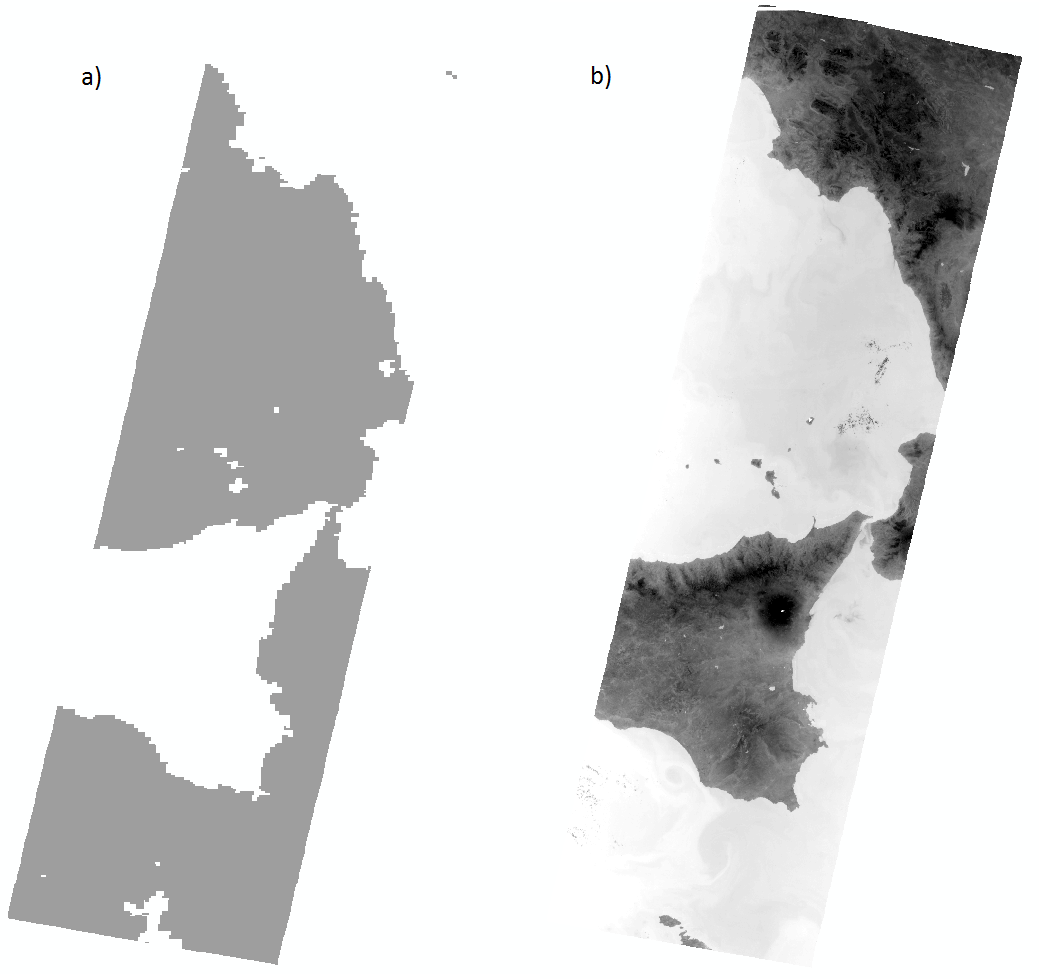
\includegraphics[width=0.6\textwidth]{SST.png}
\caption{a) MODIS SST. b) MITIP temperature product: surface temperature map in MIR band}
\label{fig:SST}

\centering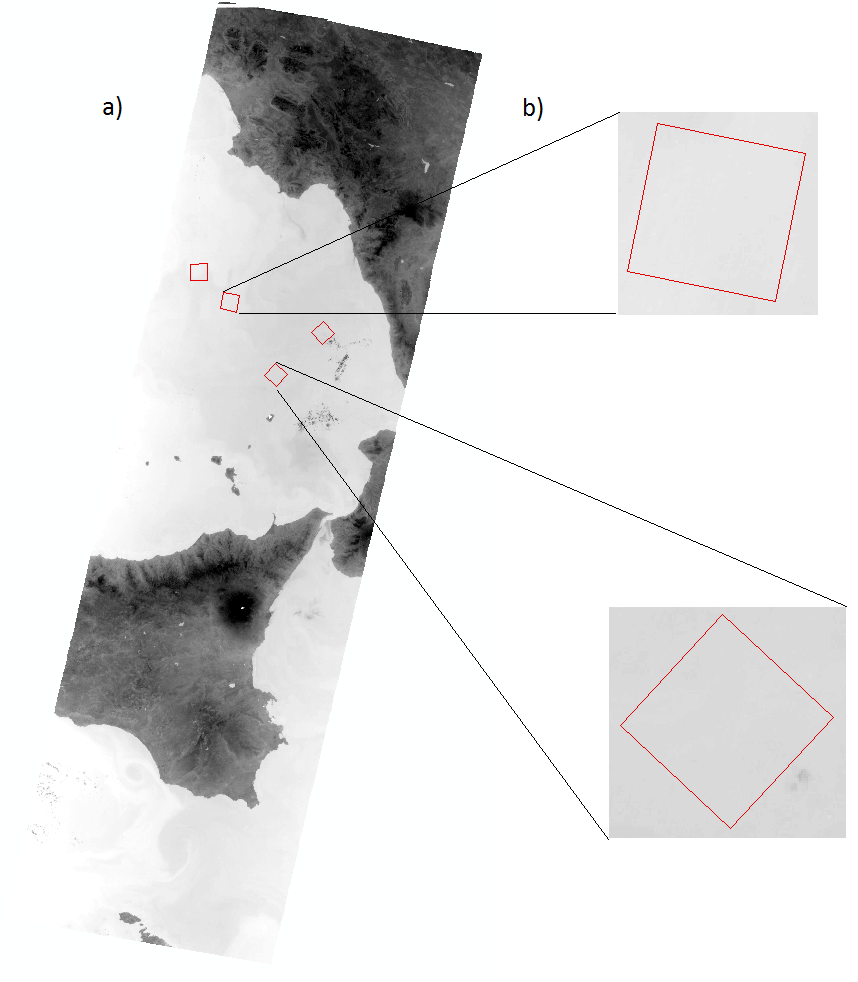
\includegraphics[width=0.6\textwidth]{selectedArea.png}
\caption{a) Selected sub-areas distribution over MITIP surface temperature in MIR band. b) Zoomed-in pictures of two sub-areas}
\label{fig:selectedArea}
\end{figure}

\begin{figure}[!htbp]
\centering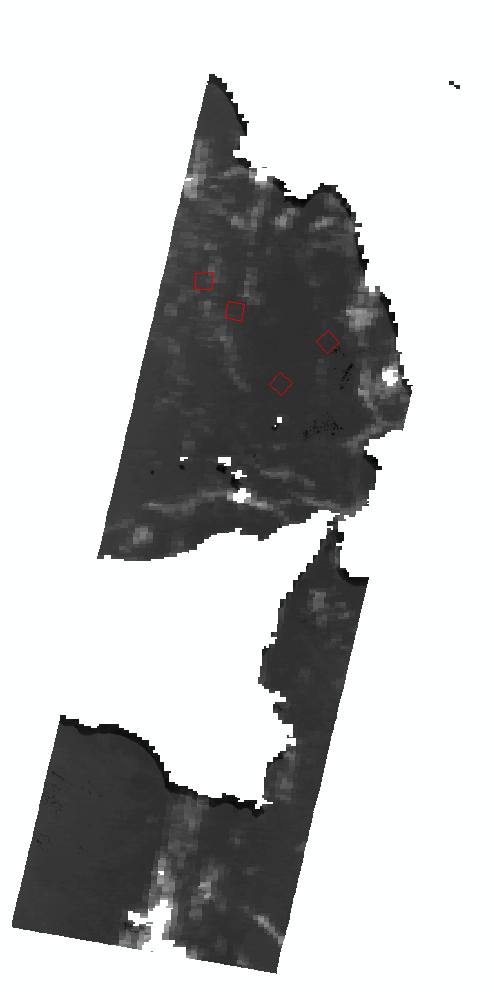
\includegraphics[width=0.4\textwidth]{differences.png}
\caption{Difference map between MODIS SST and MITIP surface temperature in MIR band}
\label{fig:Diff}
\end{figure}

%-----------------------------------
%	SUBSECTION 2
%-----------------------------------

\subsection{Results comparision with MODIS SST and calibration}
Before doing the comparison betwen MODIS SST and MITIP surface temperature products, one problem needs to be solved is that the choice of emissivity. The emissivity map derived from ASTER Global Emissivity Database is consisted of 5 bands and there are two bands, namely band 11 with wavelength 8.6 $\mu$m and band 12 with wavelength 9.1 $\mu$m fall in TET-1 imagery's TIR band with spectral range 8.5 $\mu$m to 9.3 $\mu$m {Reference}. So there comes a problem which band of emissivity map should be used.

%-----------------------------------
%	SUBSECTION 3
%-----------------------------------

% \subsection{Calibrations}

%-----------------------------------
%	SUBSECTION 3
%-----------------------------------

\subsection{transferability test (SST)}

%-----------------------------------
%	SUBSECTION 4
%-----------------------------------

\subsection{Results comparision with MODIS LST and calibration}

%-----------------------------------
%	SUBSECTION 5
%-----------------------------------

\subsection{transferability test (LST)}

%----------------------------------------------------------------------------------------
%	SECTION 2
%----------------------------------------------------------------------------------------

\section{Conclusion of the comparisons and calibrations}

%-----------------------------------
%	SUBSECTION 1
%-----------------------------------

% \subsection{Data preparasion}

%-----------------------------------
%	SUBSECTION 2
%-----------------------------------

% \subsection{Outcomes of the mitip and results comparision with MODIS LST}

%-----------------------------------
%	SUBSECTION 3
%-----------------------------------

% \subsection{Calibrations}

%-----------------------------------
%	SUBSECTION 4
%-----------------------------------

% \subsection{Test of the results of calibrations}

